\documentclass{standalone}
\usepackage{tikz}

\begin{document}

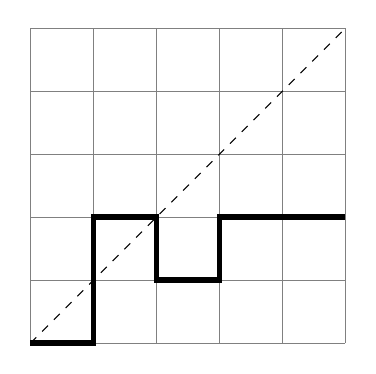
\begin{tikzpicture}[scale=0.8]
    (0,0) rectangle +(5,5);
    \draw[help lines] (0,0) grid +(5,5);
    \draw[dashed] (0,0) -- +(5,5);
    \coordinate (prev) at (0,0);
    \draw [color=black, line width=2] (0,0)--(1,0)--(1,1)--(1,2)--(2,2)--(2,1)--(3,1)--(3,2)--(4,2)--(5,2);
    % \draw (10,1) node [scale=0.5, circle, draw,fill=blue]{};

\end{tikzpicture}

\end{document}